\chapter{Domain Adaptation}
\graphicspath{{figs/2c/}}
\begin{figure}[H]
    \centering
    \begin{subfigure}{.5\textwidth}
        \centering
        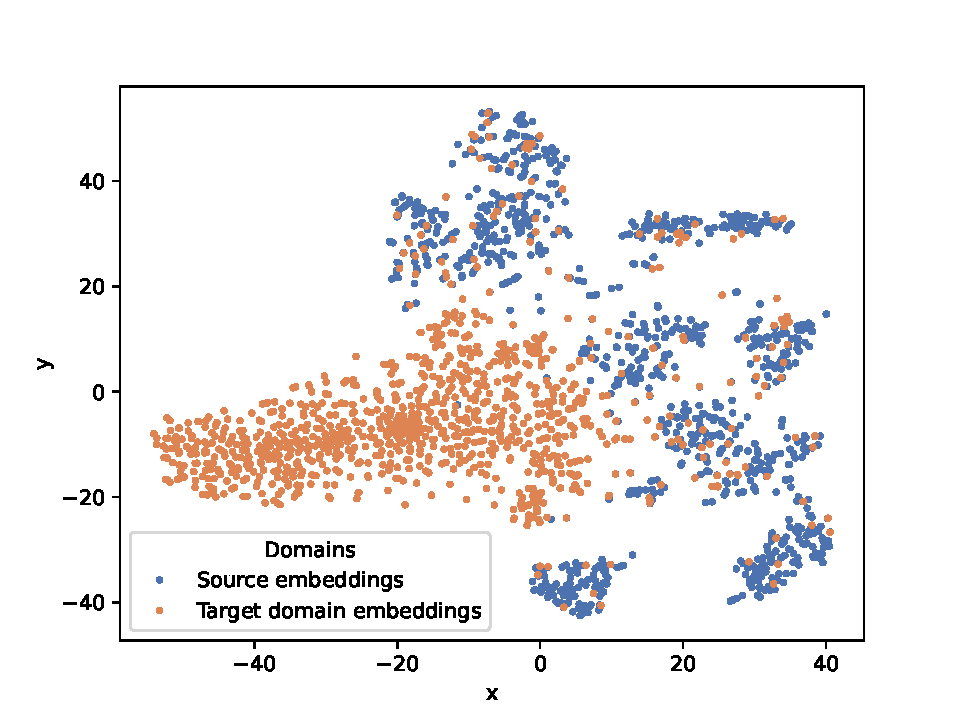
\includegraphics[width=\linewidth]{t-SNE_without_domain_adaptation.pdf}
        \caption{}
        \label{fig:t-SNE:without}
    \end{subfigure}%
    \begin{subfigure}{.5\textwidth}
        \centering
        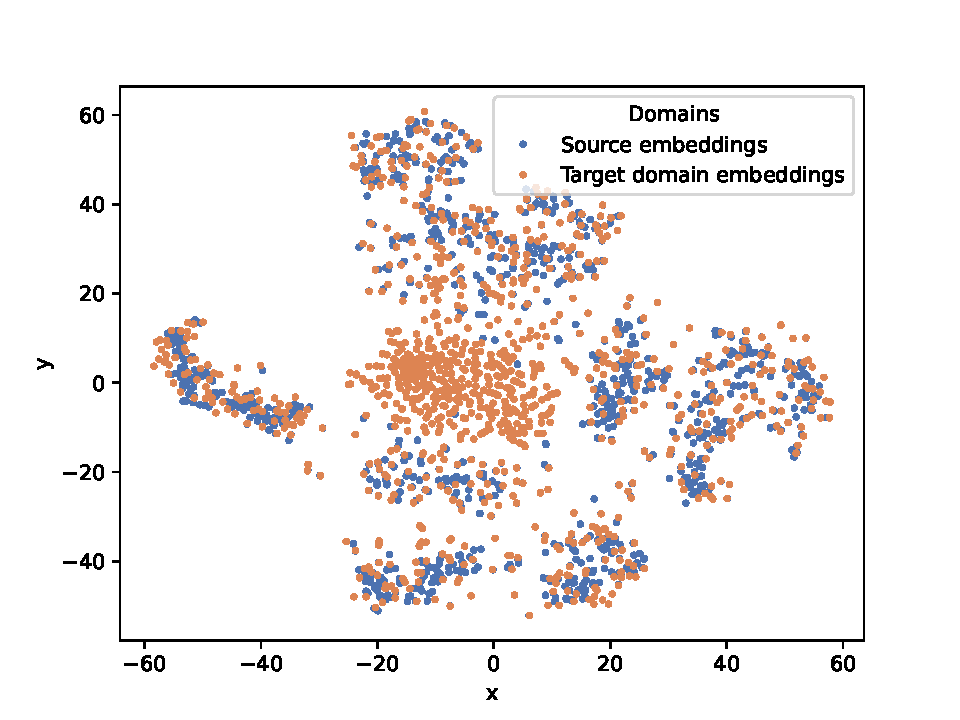
\includegraphics[width=\linewidth]{t-SNE_with_domain_adaptation.pdf}
        \caption{}
        \label{fig:t-SNE:with}
    \end{subfigure}
    \caption{t-SNE visualization of the feature extractor latent space: (a) for a baseline network without domain adaptation training. (b) for a DANN (Domain-Adversarial Neural Network) after domain adaptation training.}
    \label{fig:t-SNE}
\end{figure}

This exploration focuses on domain adaptation to tackle the task of applying models trained in one domain to a distinct yet related domain. This entails the comprehension and application of concepts like the DANN model and the Gradient Reversal Layer, which serve as tools to render a model agnostic to the domain. This practical exercise underscores the complexities of training a model on one dataset, such as labeled MNIST, and subsequently utilizing it effectively on a different dataset, such as unlabeled MNIST-M. This mirrors real-world situations where domain adaptation plays a crucial role, e.g. autonomous driving.

\paragraph*{1. If you keep the network with the three parts (green, blue, pink) but didn't use the GRL, what would happen?}

The gradient of the domain classifier is directed in a way that aids it in distinguishing between features from the source and target domains. In the absence of the Gradient Reversal Layer (GRL), the gradient would be propagated to the feature extractor, encouraging it to assist the domain classifier in distinguishing between source and target domain features. This would result in a model that becomes more domain-specific rather than domain-generalized, as it would enable the domain classifier to excel at discriminating between source and target domains, contradicting the goal of domain adaptation.

To address this issue, we employ a simple technique: we reverse the sign of the gradient, causing it to move in the opposite direction. This reversal helps the feature extractor generate domain-agnostic features, aligning with the objective of achieving domain adaptation.


\paragraph*{2. Why does the performance on the source dataset may degrade a bit?}

During our experimentation, we saw the source domain accuracy go from 99.07\% to 98.64\% and the target domain accuracy going from 53.52\% to 78.85\%. The minor performance decrease on the source dataset result from the model adapting to features common to both domains, slightly reducing its specificity for the source domain.

After 100 epochs, we a achived a target domain accuracy of 80\%, keeping the source domain accuracy at 98.5\%. The domain discriminator had an accuracy of 49\%.

% From the pratical: The gradient of the domain classifier should help to better classify the domain. Therefore if we reverse it before the end of the features extractor, we will force this CNN to do the opposite: to make the features as agnostic as possible from the domain. Which would mean that the features of MNIST and MNIST-M will be similar and only the digit info will be kept.

\paragraph*{3. Discuss the influence of the value of the negative number used to reverse the gradient in the GRL.}

The gradient reversal value balances learning domain-specific features and generalizing across domains. An optimal value is crucial for effective learning without compromising performance on either domain.

The practical propose to use a modified version of the original DANN paper's scheduler for the GRL (Gradient Reversal Layer) value, defined as 
\begin{align*}
    &\text{Our version} && \text{DANN Paper version}\\
    &f: \mathbb{N} \to [0,1] &&g: \mathbb{N} \to [0,1]\\
    &x \mapsto \frac{2}{(1 + \exp({-2\frac{x}{n}}))} - 1 && x \mapsto \frac{2}{(1 + \exp({-10 \frac{x}{n}}))} - 1
\end{align*}
where $n$ represents the number of training iterations (number of images multiplied by the number of epochs). The ratio $\frac{x}{n}$ is denoted as $p$ in the original paper, representing the training progress linearly changing from 0 to 1. The only difference between the two versions is the scalar value $2$ or $10$, which we can denote as $c$.

As an experiment, we attempted to vary $c$ within the range of $1$ to $9$. The results are presented in Figure \ref{fig:glr}, which illustrates the accuracy of DANN on the target domain after 30 epochs. 
As is common in many adversarial training setups, it's worth noting that training can sometimes exhibit random failures or instability. We reran the experiment a second time, and it appears that higher values of $c$ tend to introduce instability in the training process, resulting in more failures. Further experiments may be necessary to confirm this observation. We also attempted to use $c=10$ as in the original paper, but the training still experienced failures. Additional tuning is required to gain a better understanding of this parameter.

As a baseline experiment, we also tried directly using $-1$ as the GRL factor. However, this approach resulted in poor performance, with only a 45\% accuracy on the target domain after 20 epochs.

Please note that the performance and stability of adversarial training can be highly dependent on the specific dataset, model architecture, and other hyperparameters, so further experimentation and fine-tuning may be necessary to achieve optimal results.

\begin{figure}[H]
    \centering
    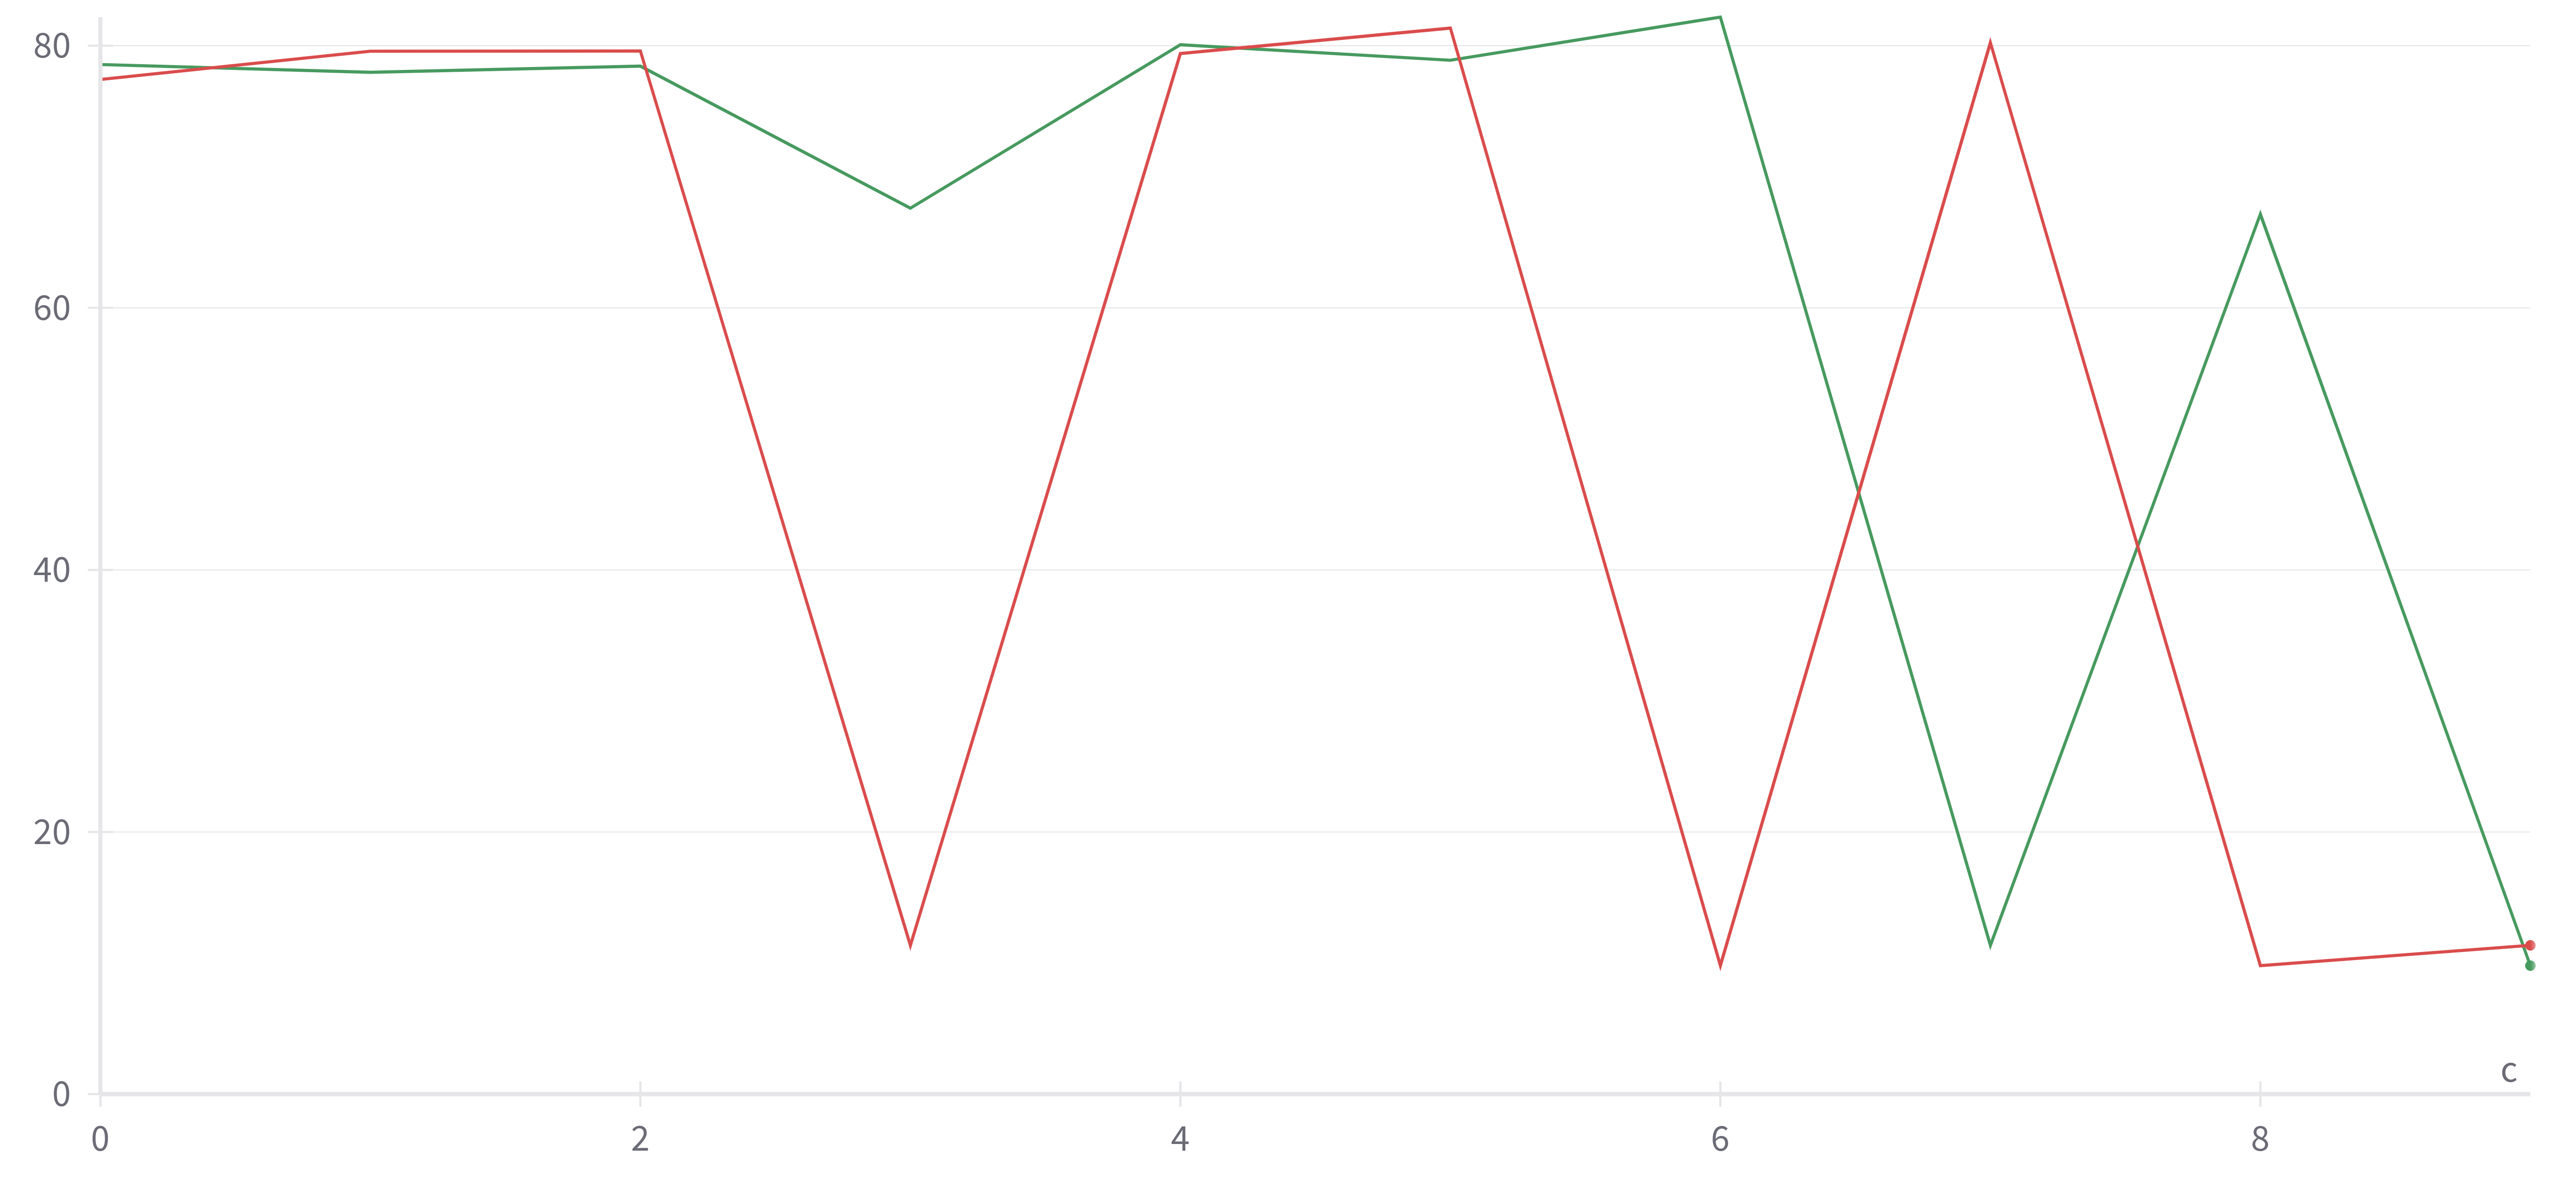
\includegraphics[width=.8\textwidth]{GLR_factor_exp.png}
    \caption{Final class accuracy on the target domain in function of $c$ for two runs. An augmentation of $c$ seem to create instability in training but further run might be needed.}
    \label{fig:glr}
\end{figure}

% GRL Factor pratical scheduling
% [SOURCE] Class loss/acc: 0.04871 / 98.44%, Domain loss/acc: 0.55289 / 75.14%
% [TARGET] Class loss/acc: 0.97395 / 74.76%, Domain loss/acc: 0.57243 / 62.88%

% GRL factor paper scheduling => Le training a failled, need rerun
% [SOURCE] Class loss/acc: 2.30145 / 11.35%, Domain loss/acc: 0.00128 / 99.99%
% [TARGET] Class loss/acc: 3.61987 / 22.76%, Domain loss/acc: 0.10717 / 97.39%

% GRL factor : -1 forall
% Epoch [1/20], GRL factor [-1.000]:   0%|          | 0/18760 [00:00<?, ?batch/s]
% Epoch [20/20], GRL factor [-1.000]: 100%|██████████| 18760/18760 [05:14<00:00, 59.62batch/s, class loss=0.00104, domain loss=1e-5]
% [SOURCE] Class loss/acc: 0.02873 / 99.19%, Domain loss/acc: 1e-05 / 100.0%
% [TARGET] Class loss/acc: 3.48452 / 45.25%, Domain loss/acc: 0.00115 / 99.95%

% 100 epoch
% GRL factor 0.7573623242165262
% Epoch 99, class loss: 0.0117, domain loss: 0.30571
% [SOURCE] Class loss/acc: 0.06666 / 98.51%, Domain loss/acc: 0.56035 / 79.72%
% [TARGET] Class loss/acc: 1.02656 / 80.01%, Domain loss/acc: 0.6842 / 49.09%


\paragraph*{4. Another common method in domain adaptation is pseudo-labeling. Investigate what it is and describe it in your own words.}

Pseudo-labeling involves generating labels for the target domain using the model's predictions. These labels are then used for further training, helping the model adapt to the target domain by leveraging its existing knowledge and narrowing the domain gap.

We attempted to implement a basic pseudo-labeling method, but unfortunately, it did not yield significant improvements. The accuracy remained relatively constant over 20 pseudo-labeling iterations. While further tuning may be necessary, we also suspect that the presence of both correct and incorrect labels may counterbalance each other, hindering the model's improvement.

\begin{figure}[htbp]
    \centering
    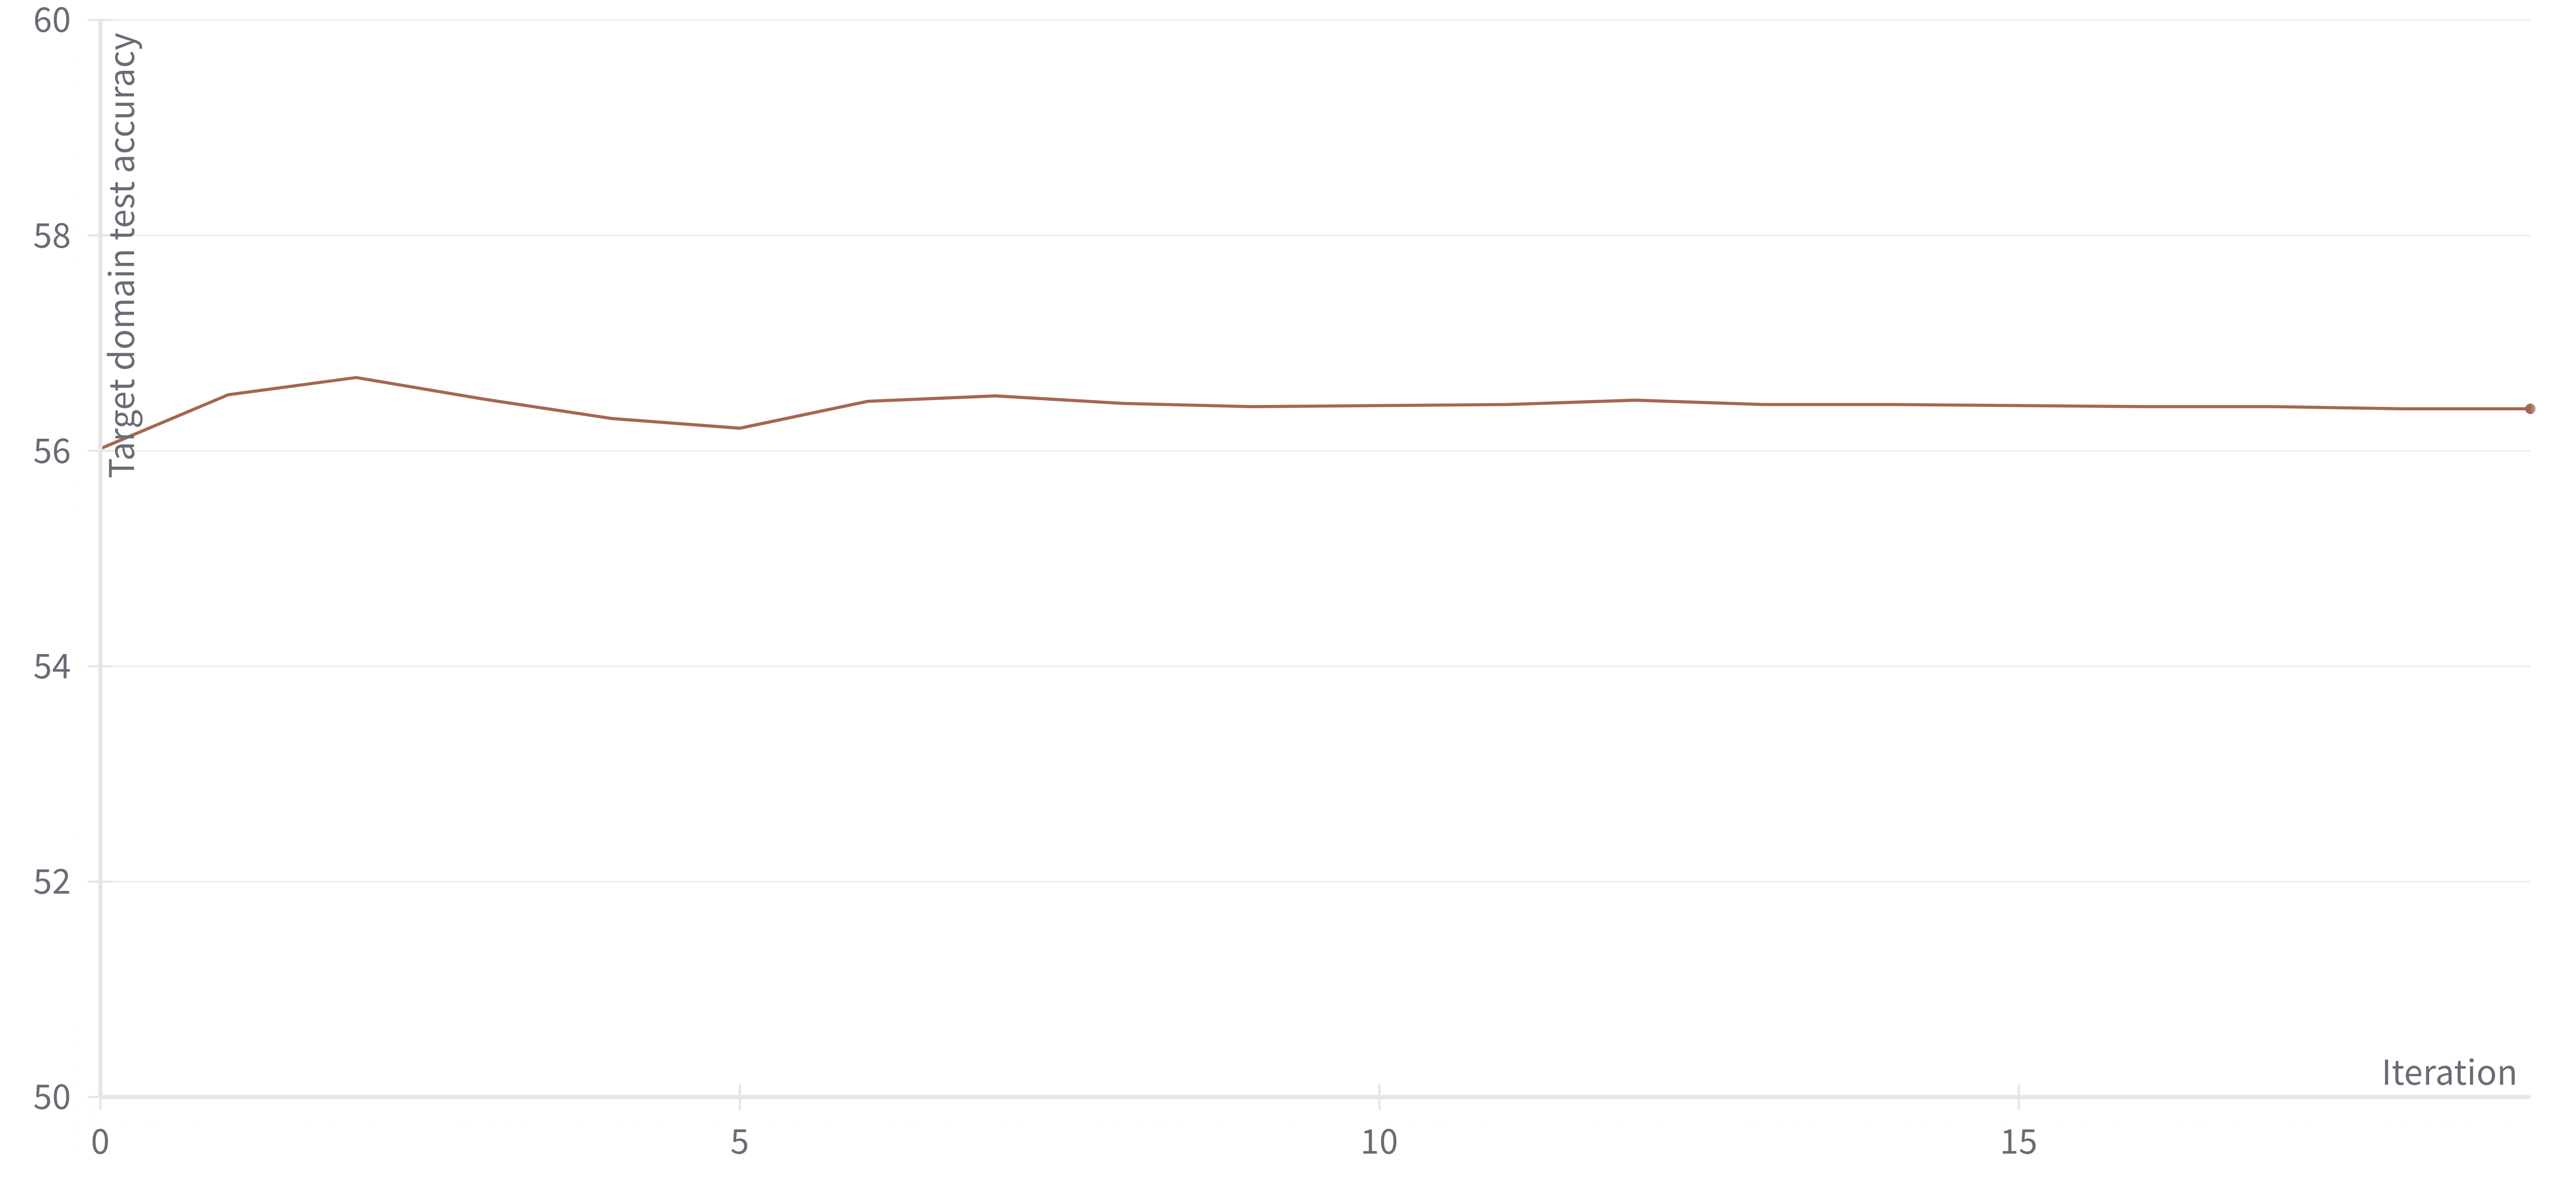
\includegraphics[width=.8\textwidth]{pseudo_labeling.png}
    \caption{Accuracy on the target domain's test dataset at each pseudo-labeling iteration is being monitored. The model's improvement appears to be very limited, potentially because the balance between correct and incorrect labeling tends to average out.}
    \label{fig:pseudo_labeling}
\end{figure}

% TODO: Ultra court, faut que je repasse sur le TME, peut-être mettre une figure qui montre qu'on classifie bien colorMNIST + ajouter la visualisation des espaces latents?

